\section{Supplemental Materials}

\subsection{Simulation and Analysis Code Available Online}
All of the simulation and analysis code for generating the figures in this paper is available online.  To find the source code please visit our Github repository at 

https://github.com/wmcfadden/activnet

\subsection{Steady-state Approximation of Effective Viscosity}
\label{sec:eff_vic}
We begin with a calculation of a strain rate estimate of the effective viscosity for a network described by our model in the limit of highly rigid filaments.  We carry this out by assuming we have applied a constant stress along a transect of the network.  With moderate stresses, we assume the network reaches a steady state affine creep. In this situation, we would find that the stress in the network exactly balances the sum of the drag-like forces from cross-link slip.  So for any transect of length D, we have a force balance equation.

\begin{equation}
	\mathbf{\sigma} = \frac{1}{D}\sum_{filaments}\: \sum_{crosslinks}\xi \cdot (\mathbf{v_i(x)}-\mathbf{v_j(x)})
\end{equation}

where $\mathbf{v_i(x)}-\mathbf{v_j(x)}$ is the difference between the velocity of a filament, $i$, and the velocity of the filament, $j$, to which it is attached at the cross-link location, $\mathbf{x}$. We can convert the sum over cross-links to an integral over the length using the average density of cross-links, $1/l_c$ and invoking the assumption of (linear order) affine strain rate, $\mathbf{v_i(x)}-\mathbf{v_j(x)}=\dot \gamma x$. This results in

\begin{multline}
	\mathbf{\sigma} =  \frac{1}{D}\sum_{filaments}\:  \int_0^L \xi \cdot  \: (\mathbf{v_i(s)}-\mathbf{v_j(s)}) \:\frac{ds \cos \theta }{l_c} \\
	= \sum_{filaments}\:  \frac{\xi \dot \gamma L}{l_c} \cos \theta \cdot (x_l + \frac{L}{2} \cos \theta)
\end{multline}

Here we have introduced the variables $x_l$, and $\theta$ to describe the leftmost endpoint and the angular orientation of a given filament respectively.  Next, to perform the sum over all filaments we convert this to an integral over all orientations and endpoints that intersect our line of stress. We assume for simplicity that filament stretch and filament alignment are negligible in this low strain approximation.  Therefore, the max distance for the leftmost endpoint is the length of a filament, L, and the maximum angle as a function of endpoint is $\arccos(x_l/L)$.  The linear density of endpoints is the constant $D/l_cL$ so our integrals can be rewritten as this density over $x_l$ and $\theta$ between our maximum and minimum allowed bounds.

\begin{equation}
	\mathbf{\sigma} =  \frac{1}{D} \int_0^L dx_l \int_{-\arccos (\frac{x_l}{L})}^{\arccos (\frac{x_l}{L})}\pi d\theta \frac{\xi \dot \gamma L}{l_c} \cdot \frac{D}{Ll_c}\cdot (x_l \cos \theta + \frac{L}{2} cos^2\theta)
\end{equation}

Carrying out the integrals and correcting for dangling filament ends leaves us with a relation between stress and strain rate.

\begin{equation}
	\mathbf{\sigma} = 4 \pi \left ( \frac{ L}{l_c}-1 \right)^2 \xi \dot \gamma 
\end{equation}

We recognize the constant of proportionality between stress and strain rate as a viscosity (in 2 dimensions).  Therefore, our approximation for the effective viscosity, $\eta_{c}$, at steady state creep in this low strain limit is

\begin{equation}
	\label{lin_eqn}
	\mathbf{\sigma} = 4 \pi \left ( \frac{ L}{l_c}-1 \right)^2 \xi
\end{equation}



\subsection{Critical filament lifetime for steady state filament extension}
We seek to determine a critical filament lifetime, $\tau_{crit}$ , below which the density of filaments approaches a stable steady state under constant extensional strain. To this end, let $\rho$ be the filament density (i.e. number of filaments per unit area). We consider a simple coarse grained model for how $\rho$ changes as a function of filament assembly $k_{ass}$, filament disassembly $k_{diss}$, $\rho$ and strain thinning $\dot{\gamma}\rho$. Using $\rho_0 = \frac{k_{ass}}{k_{diss}}$, $\tau_r=\frac{1}{k_{diss}}$, and $\dot{\gamma}=\frac{\sigma}{\eta_c}$.

\begin{equation}
	\label{drho_1}
	\frac{d\rho}{dt}=\frac{1}{\tau_r}\left ( \rho_0 - \rho - \frac{\sigma \tau_r}{\eta_c(\rho)} \rho\right )
\end{equation}

where $\eta_c = \eta_c(\rho)$ on the right hand side reflects the dependence of effective viscosity on network density.  The strength of this dependence determines whether there exists a stable steady state, representing continuous flow.  Using $\eta_c(\rho)\sim \xi \left ( \frac{L}{l_c(\rho)} -1 \right )^2$ from above (ignoring the numerical prefactor) and $\rho \sim \frac{2}{L l_c(\rho)}$, we obtain:


\begin{equation}
	\label{drho_2}
	\frac{d\rho}{dt}=\frac{1}{\tau_r}\left ( \rho_0 - \rho - \frac{\sigma \tau_r}{\xi(\rho L^2/2 -1)^2}\rho\right )
\end{equation}

\begin{figure}[H]
	\centering
	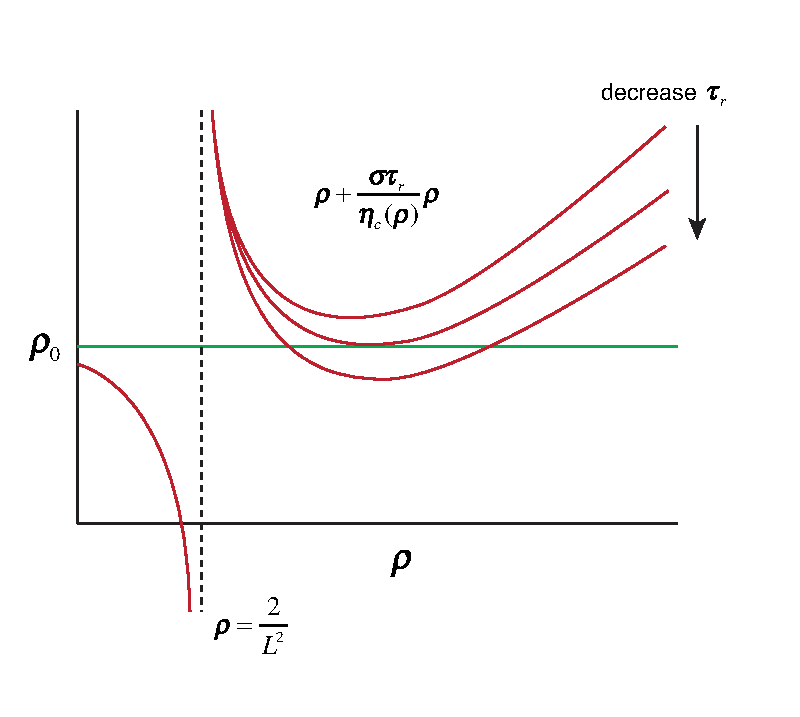
\includegraphics[width=\hsize]{active/figures/FigS0}
	\caption{\label{fig:flux_balance}  Flux balance analysis of network density. Qualitative plots of $\rho+\frac{\sigma \tau_r}{\eta_c(\rho)}\rho$ (red curves) vs $\rho_0$ (green line) for different values of $\tau_r$.  For sufficiently large $\tau_r$, there are no crossings.  For $\tau_r < \tau_{crit}$, there are two crossings:  The rightmost crossing represents a stable steady state.  }
\end{figure}


Figure \ref{fig:flux_balance} sketches the positive ($\rho_0$) and negative ($\rho+\frac{\sigma \tau_r}{\eta_c(\rho)}\rho$) contributions to the right hand side of Equation 6 for different values of $\tau_r$. For sufficiently large $\tau_r$, there is no stable state, i.e. strain thinning will occur.  However, as $\tau_r$ decreases below a critical value $\tau_{crit}$, a stable steady state appears.  Note that when $\tau_r = \tau_{crit}$, $\rho+\frac{\sigma\tau_r}{\eta_c(\rho)}\rho$ passes through a minimum value $\rho_0$ at $\rho=\rho^*$.  Accordingly, to determine $\tau_{crit}$, we solve:

\begin{equation}
	\label{drho_3}
	0 = \frac{d}{d\rho}\left( \rho + \frac{\sigma\tau_r}{\eta_c(\rho)} \rho\right ) = 1 - \frac{\sigma\tau_r}{\xi (\rho L^2/2-1)^3}
\end{equation}

From this, with some algebra, we infer that

\begin{equation}
	\label{drho_4}
	\rho^* = \frac{2}{L^2}\left ( 1 + \left( \frac{\sigma\tau_r}{\xi}\right )^{1/3} \right )
\end{equation}

and 

\begin{equation}
	\label{drho_5}
	\frac{\sigma\tau_r}{\eta_c(\rho^*)} =  \left( \frac{\sigma\tau_r}{\xi}\right )^{1/3} 
\end{equation}

We seek a value for $\tau_r=\tau_{crit}$ at which


\begin{equation}
	\label{drho_6}
	\rho^* + \frac{\sigma\tau_{crit}}{\eta_c(\rho^*)}\rho^* =  \rho_0
\end{equation}

Substituting from above, and using $\rho_0=\frac{2}{L l_c}$, we have:

\begin{equation}
	\label{drho_7}
	\frac{2}{L^2}\left ( 1 + \left( \frac{\sigma\tau_{crit}}{\xi}\right )^{1/3}  \right )
	\left ( 1 + \left( \frac{\sigma\tau_{crit}}{\xi}\right )^{1/3}  \right )
	= \frac{2}{L l_c}
\end{equation}

Finally, rearranging terms, we obtain

\begin{equation}
	\label{drho_8}
	\tau_{crit}=\frac{\xi}{\sigma}\left( \sqrt{\frac{L}{l_c}}-1\right )^3
\end{equation}



\begin{sidewaystable}[h]
		\centering
		\caption{Simulation Parameter Values}
		\label{table:para2}
		\begin{tabular}{|c|ccccccc|}
			\hline
			Parameter     & \textbf{Fig 3}          & \textbf{Fig 4}       & \textbf{Fig S2a,b}    & \textbf{Fig S2c,d}     & \textbf{Fig 7}    & \textbf{Fig 9}          \\ \hline
			$L$           & $1,3,5,7,10$      & $3$             & $3,5$         & $3,5$                 & $5$         & $3,5,8$            \\ 
			$l_c$         & $0.2,0.3,0.5,0.8$ & $0.3,0.5$       & $0.3$       & $0.15,0.2,0.3,0.4$ & $0.2,0.3$        & $0.15,0.2,0.3,0.4$ \\ 
			$\mu_e/\mu_c$ & $100$             & $100$           & $3-300$     & $100$     & $100$           & $100$              \\ 
			$\mu_c$       & $0.01$            & $0.01$          & $0.01-0.3$  & $0.001-0.03$       & $0.01$      & $0.01$             \\ 
			$\xi$         & $0.1,1$          & $0.05,0.1,1$      & $0.01,0.1,1$  & $0.1,1$  & $0.1,1,3.3$   & $0.1,1$           \\ 
			$\upsilon$    & ~                 & ~               & $0.1,0.3,1$ & $0.1,1$   & $0.1,1,3$    & $0.1$              \\ 
			$\phi$        & ~                 & ~               & $0.25$      & $0.5$     & $0.25,0.75$    & $0.25$             \\ 
			$\tau_r$      & ~                 & $0.1-10^4$      & ~           & ~         & $0.01-10^3$  & $0.01-10^3$              \\ 
			$\sigma$      & $0.0002-0.01$     & $0.00003-0.005$ & ~           & ~         & ~            & ~                          \\
			\hline
		\end{tabular}
\end{sidewaystable}


\begin{figure}[H]
	\centering
	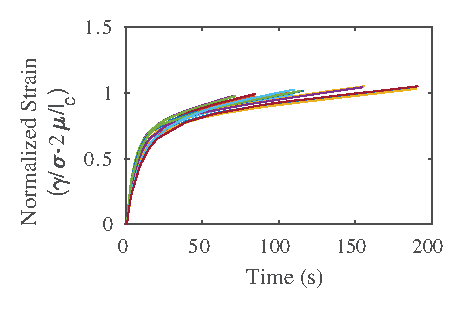
\includegraphics[width=\hsize]{active/figures/FigS1}
	\caption{\label{fig:passive_supp}  Fast viscoelastic response to extensional stress. Plots of normalized strain vs time during the elastic phase of deformation in passive networks under extensional stress.  Measured strain is normalized by the equilibrium strain predicted for a network of elastic filaments without crosslink slip $\gamma_{eq} = \sigma/G_0 = \sigma/(2\mu/l_c)$.  }
\end{figure}

\begin{figure}[H]
	\centering
	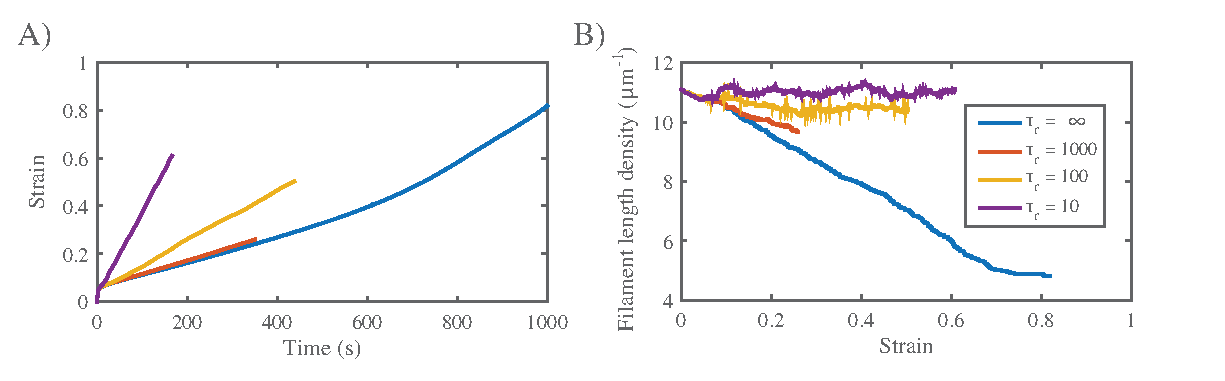
\includegraphics[width=\hsize]{active/figures/FigS2}
	\caption{\label{fig:thinning}  Filament turnover rescues strain thinning.  \textbf{a)} Plots of strain vs time for different turnover times (see inset in (b)). Note the increase in strain rates with decreasing turnover time. \textbf{b)} Plots of filament density vs strain for different turnover times $\tau_r$.  For intermediate $\tau_r$, simulations predict progressive strain thinning, but at a lower rate than in the complete absence of recycling. For higher $\tau_r$, densities approach steady state values at longer times.  }
\end{figure}

\begin{figure}[H]
	\centering
	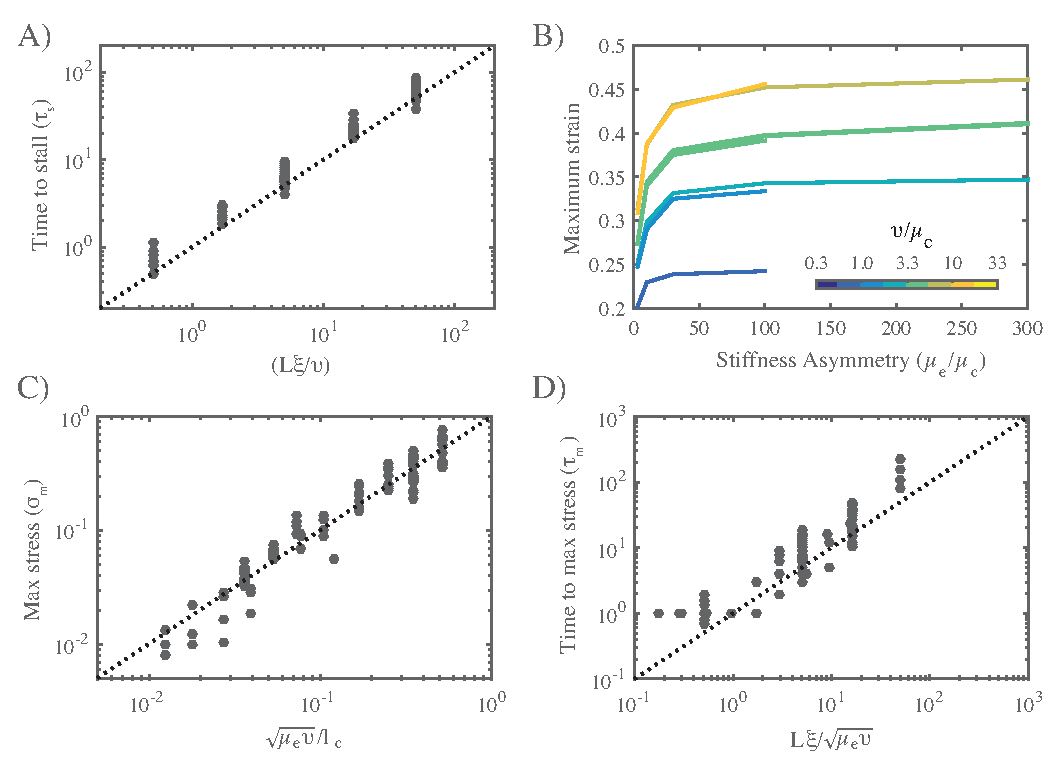
\includegraphics[width=\hsize]{active/figures/FigS3}
	\caption{\label{fig:active_supp}  Mechanical properties of active networks.  \textbf{a)}  Time for freely contracting networks to reach maximum strain, $\tau_s$, scales with $L\xi/\upsilon$.  \textbf{b)} Free contraction requires asymmetric filament compliance, and total network strain increases with the applied myosin force $\upsilon$. Note that the maximum contraction approaches an asymptotic limit as the stiffness asymmetry approaches a ratio of $\sim 100$.   \textbf{c)}  Maximum stress achieved during isometric contraction, $\sigma_m$, scales approximately with $\sqrt{\mu_e\upsilon}/l_c$.  \textbf{d)} Time to reach max stress during isometric contraction scales approximately with $L\xi/\sqrt{\mu_e\upsilon}$. Scalings for $\tau_s$, $\sigma_m$ and $\tau_m$ were determined empirically by trial and error, guided by dimensional analysis. }
\end{figure}

\begin{figure}[H]
	\centering
	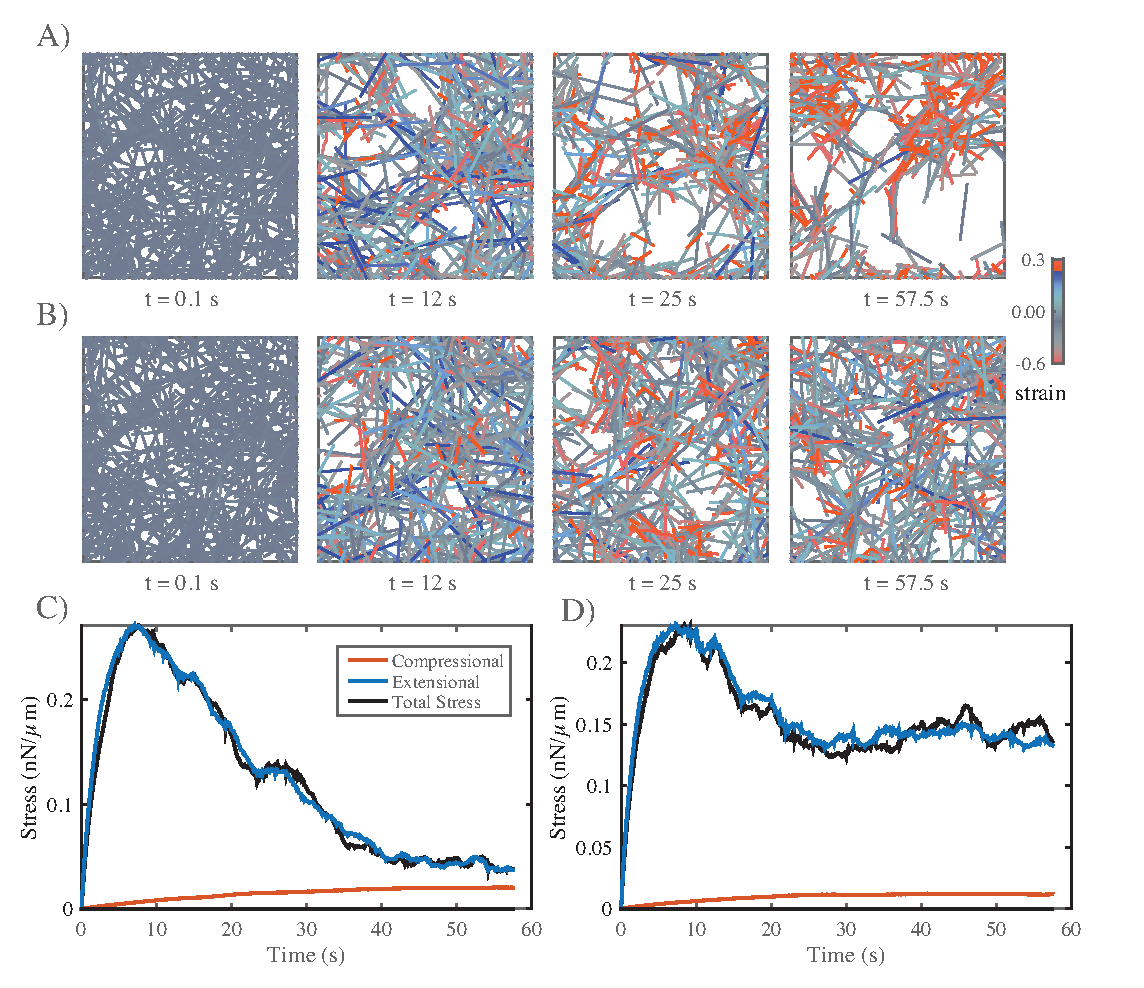
\includegraphics[width=\hsize]{active/figures/FigS4}
	\caption{\label{fig:active_tear}  Filament turnover prevents tearing of active networks.  \textbf{a)}  An active network undergoing large scale deformations due to active filament rearrangements.  \textbf{b)}  The same network as in (a) but with a shorter filament turnover time.  \textbf{c)}  Plots of internal stress vs time for the network in (a).  \textbf{d)}  Plots of internal stress vs time for the network in (b).  }
\end{figure}

\begin{figure}[H]
	\centering
	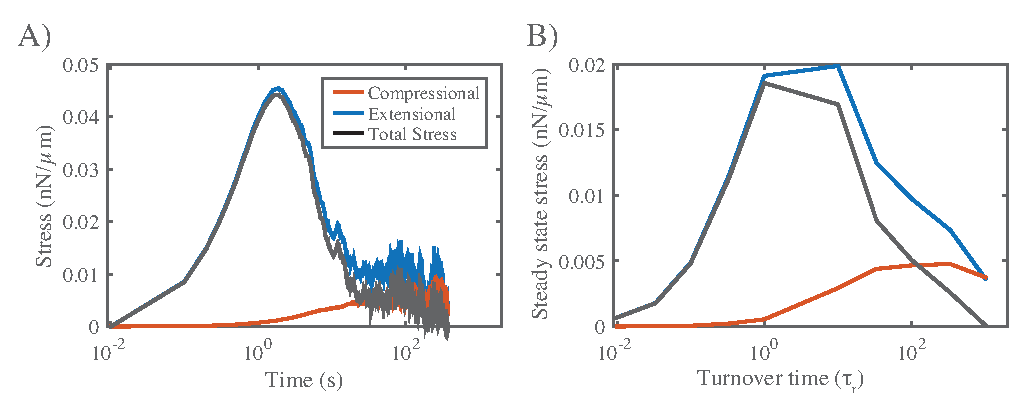
\includegraphics[width=\hsize]{active/figures/FigS5}
	\caption{\label{fig:recycle_supp}  Bimodal dependence on turnover time matches bimodal buildup and dissipation of stress in the absence of turnover.  \textbf{a)}  Bimodal buildup of stress in a network with very slow turnover ($\tau_r = 1000s$).  \textbf{b)}  Steady state stress for networks with same parameters as in (a), but  for a range of filament turnover times.   }
\end{figure}

\begin{figure}[H]
	\centering
	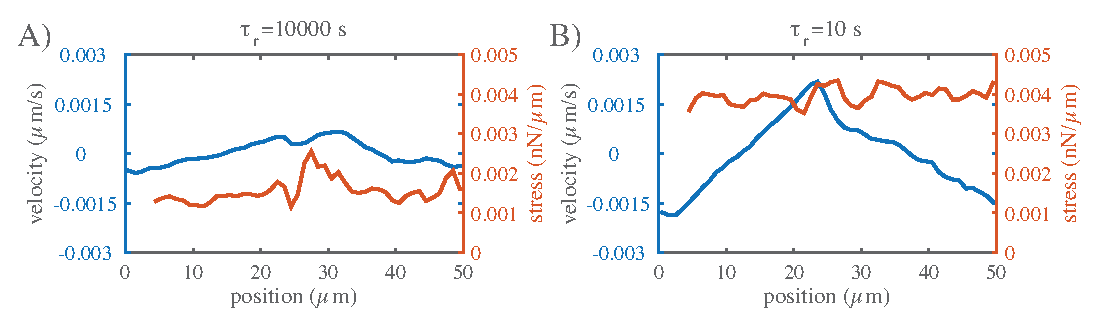
\includegraphics[width=\hsize]{active/figures/FigS6}
	\caption{\label{fig:combo_prof}  Dynamics of steady state flow. Plots of stress and strain vs position for networks in which motor activity is limited to the right-half domain and filament turnover time is either  \textbf{a)} $\tau_r = 10000$ or  \textbf{b)} $\tau_r = 10 s$.  Blue indicates velocity while orange represents total stress, measured as described in the main text. }
\end{figure}